\chapter{[Por revisar] Marco teórico y contexto tecnológico}
\label{chapter:marco_teorico}

\chapquote{Una vez que algo es una pasión, hay motivación.}{Michael Schumacher}

En este capítulo se introducen los conceptos teóricos sobre los que se asienta el desarrollo de este proyecto. Con el contenido de este capítulo se espera crear un base de conocimiento sobre la que desarrollar el resto de este documento. Además, se realiza un análisis de las herramientas que se van a emplear para desarrollar el sistema y cómo estas se encuadran en el contexto tecnológico actual.

\section{Marco teórico}
    \label{section:marco_teorico}

    En el capítulo anterior se realizó una introducción a la salud mental y a su impacto actual en la sociedad, tomando esta sección el testigo para introducir al lector en los trastornos concretos que serán tratados a lo largo de todo el proyecto: estrés, depresión y soledad, junto a la relación de estas con el suicidio.

    No obstante, antes de comenzar con las enfermedades\footnote{A lo largo del documento se utilizarán los términos enfermedad, trastorno o desorden indistintamente para aliviar la notación.} concretas, conviene especificar previamente lo que se entiende por desorden mental. Según \cite{ortega_gonzalez_enfermedades_2021}, \textit{``desde el punto de vista clínico, la enfermedad mental debe de poseer una serie de características que permita identificarla para su posterior diagnóstico''}. Asimismo, \textit{``una enfermedad mental o trastorno mental debe afectar al individuo de forma parcial o íntegra con respecto a diferentes capacidades y funciones cuyo desarrollo se fundamenta en el cerebro y la mente. Este tipo de enfermedades conllevan una respuesta anómala que trasciende las respuestas culturales normalizadas, como puede ser desarrollar un trastorno depresivo a raíz de una ruptura''}.

    Por tanto, para cada trastorno se detallarán las características que permiten identificarlas y cómo se manifiestan en los individuos, si bien estas respuestas pueden variar notablemente entre individuos. Asimismo, para profundizar en estas cuestiones se anima al lector a acudir a la bibliografía que será citada, o bien a la \textit{Clasificación Internacional de Enfermedades} de la \gls{oms} \cite{oms_clasificacion_nodate} o al \textit{Manual Diagnóstico y Estadístico de los Trastornos Mentales} de la \gls{apa} \cite{american_psychological_association_manual_2014}, dos publicaciones de referencia que ahondan profundamente en los criterios de diagnóstico de salud mental.

    \subsection{Estrés}
        La \gls{oms} define el estrés como \textit{``el conjunto de reacciones fisiológicas que prepara el organismo para la acción''} \cite{torrades_estres_2007}, tratándose en primera instancia de un sistema de alerta ante situaciones desafiantes o amenazantes necesario para la supervivencia. La presencia del estrés depende del estado físico y psíquico de cada persona, pero algunas situaciones que lo pueden provocar son, entre otras: cambiar de trabajo, hablar en público, o mudarse de vivienda. Se estima que nueve de cada diez personas han sentido estrés en el último año y un 40\% de la población lo sufre de forma continua \cite{nogera_mas_estres_2024}.
        
        Este mecanismo cual estimula el organismo para que éste alcance su objetivo. Debido a esta caracterización, este momento es conocido como fase de alerta, y es la primera etapa del estrés. Una vez que el estímulo ha cesado, el organismo vuelve a su estado habitual (también conocido como basal).
        
        No obstante, el problema radica esa presión no desaparece y el individuo entra en una segunda fase, conocida como estado de resistencia. \textit{``Cuando ciertas circunstancias, como la sobrecarga de trabajo, las presiones económicas o sociales, o un ambiente competitivo, se perciben inconscientemente como una «amenaza», se empieza a tener una sensación de incomodidad. Cuando esta sensación se mantiene en el tiempo, se puede llegar a un estado de agotamiento, con posibles alteraciones funcionales y orgánicas''} \cite{torrades_estres_2007}.

        Sin profundizar en cuestiones biológicas, en estas situaciones el organismo libera ciertas hormonas, las cuales se encargan de regular, excitar o inhibir la actividad de los diferentes órganos. Algunas de ellas son el cortisol (también conocida como ``la hormona del estrés''), o la adrenalina y la noradrenalina. 
        
        Los niveles de cortisol están asociados con \textit{``euforia y propiedades similares a la recompensa relacionadas con el comportamiento de búsqueda de sensaciones''} \cite{currid_efectos_2019}; mientras que la adrenalina y la noradrenalina se encargan de poner el cuerpo en estado de alerta y prepararlo para luchar o huir \cite{torrades_estres_2007}.

        Si el individuo está expuesto de forma prolongada a amenazas, acaban disminuyendo paulatinamente sus capacidades de respuesta; si bien puede resistir durante más tiempo. Si aún así se mantiene la situación, se llega a la última etapa, conocida fase de agotamiento, la cual consiste en \textit{`` un estado de gran deterioro, con pérdida importante de las capacidades fisiológicas, en la que el sujeto experimenta un retroceso muy considerable en sus habilidades sociales, así como en sus capacidades de adaptación e interrelación con el medio''} \cite{torrades_estres_2007}. En la Figura \ref{figure:marco_teorico:fases_estres} se representan las tres fases descritas.

        \begin{figure}[h]
            \centering
            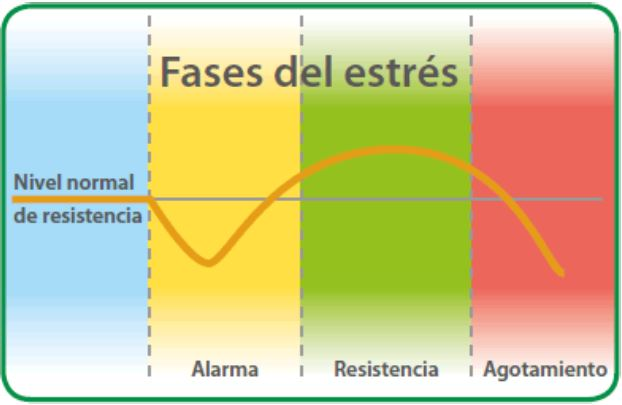
\includegraphics[width=0.66\textwidth]{figures/fases estres.JPG}
            \caption[Las tres fases del estrés]
            {Las tres fases del estrés. Imagen extraída de \cite{currid_efectos_2019}.}
            \label{figure:marco_teorico:fases_estres}
        \end{figure}

        En cuanto a las consecuencias del estrés, se pueden clasificar en tres grandes áreas: síntomas físicos, alteraciones de la conducta y alternaciones emocionales.

        Algunos de los posibles síntomas físicos son: \textit{``fatiga crónica; cefaleas y migraña; alteraciones gastrointestinales; dolores musculares; alteraciones respiratorias; alteraciones del sueño; alteraciones dermatológicas; alteraciones menstruales y disfunciones sexuales''} \cite{torrades_estres_2007}.

        En el campo de las alteraciones conductuales se puede halla: \textit{``una irregular conducta alimentaria y el abuso de drogas, fármacos y alcohol. Las conductas violentas suelen ser muy frecuentes, como la agresión, la actitud defensiva y el cinismo''} \cite{torrades_estres_2007}, mientras que a nivel emocional las más comunes son: ansiedad, irritabilidad, baja autoestima, distanciamiento emocional, falta de motivación y dificultades de concentración.

        En cuanto al diagnóstico del mismo, la \gls{pss} (o en español \textit{``Escala de Estrés Percibido''}) es el instrumento psicológico más comúnmente utilizado para medir la percepción del estrés. \textit{``Es una medida del grado en que las situaciones en la vida de una persona son valoradas como estresantes. Los artículos fueron diseñados para aprovechar la forma en que los encuestados impredecibles, incontrolables y sobrecargados encuentran sus vidas''} \cite{currid_efectos_2019}. 
        
        Por otra parte, \textit{``los elementos son fáciles de entender y las alternativas de respuesta son fáciles de entender. Además, las preguntas son de carácter general y, por lo tanto, están relativamente exentas de contenido específico para cualquier grupo de subpoblación''} \cite{cohen_global_1983}. La versión de diez preguntas de este cuestionario puede encontrarse en el Anexo \ref{cuestionarios:pss_10}.

        Por último, se pueden nombrar algunas acciones para paliar el estrés, si bien la acción recomendada en casos graves es acudir a un psicólogo.\footnote{En el transcurso de este proyecto, como se verá en secciones posteriores, se ha contado con la asesoría de dos psicólogas. Las pautas propuestas que se mostrarán a los usuarios se pueden encontrar en el Anexo \ref{chapter:recomendaciones:estres}} Según la \gls{oms} \cite{oms_estres_2023}, algunas de ellas son: 
        \begin{itemize}
            \item Seguir una rutina diaria.
            \item Dormir mucho, en particular de forma regular y limitando el uso de aparatos electrónicos antes de dormir, entre otros buenos hábitos.
            \item Realizar ejercicio con regularidad.
            \item Mantener una dieta saludable.
            \item Permanecer en contacto con los demás.
        \end{itemize}


    \subsection{Depresión}

        La depresión, también conocida como ``trastorno depresivo mayor'' o ``depresión clínica'' es una enfermedad mental que se puede describir como un estado de intensa tristeza, melancolía o desesperación, avanzada hasta perturbar el funcionamiento social o las actividades diarias de una persona \cite{van_neerven_rarrxr_2008}. Es diferente de los cambios del estado de ánimo, pudiendo afectar a todos los ámbitos de la vida, incluidas las relaciones familiares y/o de amistad \cite{oms_depresion_2023}
        
        Según la \gls{oms}, el 3,8\% de la población experimenta depresión, incluido el 5\% de los adultos (4\% entre los hombres y el 6\% entre las mujeres) y el 5,7\% de los adultos mayores de 60 años; elevándose el número de personas con depresión a aproximadamente 280 millones de personas en todo el mundo \cite{oms_depresion_2023}.

        Por otra parte, esta enfermedad se confunde comúnmente con la tristeza. La tristeza es una emoción primaria, mientras que en la depresión, \textit{``hay una disminución significativa de la funcionalidad de la persona, mientras que en la tristeza no se evidencia una alteración de la funcionalidad y de las diferentes esferas de la vida cotidiana de la persona. También en la tristeza el sentimiento displacentero es provocado por un motivo puntual y definido, mientras que la depresión no siempre tiene una causa específica para su sufrimiento, por lo que la persona deprimida no siempre sabe cuál es la razón de su depresión''} \cite{ospina_perez_entendiendo_2018}.

        Actualmente, se desconocen las causas exactas que causan la depresión, si bien, según la \gls{oms} \textit{``es el resultado de interacciones complejas entre factores sociales, psicológicos y biológicos''} \cite{oms_depresion_2023}. Se cree que pueden existir ciertos desencadenantes que incentiven la aparición de este trastorno, conocidos como factores de riesgo. Algunos de ellos son \cite{karamchandani_batra_sistema_2021}:

        \begin{itemize}
            \item Eventos estresantes, como, por ejemplo, problemas económicos, discusiones familiares o la pérdida de un ser querido \cite{tennant_life_2002}.
            \item Presencia de otras enfermedades, tanto mentales como el trastorno de Ansiedad o el \gls{tdah}; como físicas, como por ejemplo, enfermedades cardiovasculares y diabetes; o de enfermedades crónicas. 
            \item Ciertos medicamentos utilizados para tratar afecciones comunes como el asma o el acné. En particular, los que mayor riesgo representan son la \textit{Isotretinoína}, \textit{Rimonabant} y el \textit{Alpha Interferon}.
        \end{itemize}

        En cuanto a las consecuencias en los pacientes, se puede plantear la misma división que en el caso del estrés:  síntomas físicos, alteraciones de la conducta y alternaciones emocionales.
        
        Como síntomas físicos se pueden hallar, entre otros \cite{sawchuk_depresion_nodate} \cite{oms_depresion_2023}: 

        \begin{itemize}
            \item Alteraciones del sueño.
            \item Cansancio y falta de energía.    
            \item Falta de apetito y adelgazamiento.
            \item Lentitud para razonar, hablar y hacer movimientos corporales.
            \item Problemas físicos inexplicables, como dolor de espalda o de cabeza.
        \end{itemize}

        En el campo de las alteraciones conductuales se pueden encontrar  \cite{sawchuk_depresion_nodate} \cite{oms_depresion_2023}: 

        \begin{itemize}
            \item Arrebatos de enojo, irritabilidad o frustración.
            \item Pérdida de interés o placer por la mayoría o todas de las actividades habituales.
            \item Dificultad para pensar, concentrarse, tomar decisiones y recordar cosas.
        \end{itemize}
        
        Por otra parte, en cuanto a las alternaciones emocionales se pueden hallar las siguientes \cite{sawchuk_depresion_nodate} \cite{oms_depresion_2023}:

        \begin{itemize}
            \item Sentimientos de tristeza, ganas de llorar, vacío o desesperanza.
            \item Sentimientos de inutilidad o culpa excesiva, fijación en fracasos del pasado.
            \item Baja autoestima.
            \item Ansiedad, agitación o inquietud.
            \item Pensamientos frecuentes o recurrentes sobre la muerte, pensamientos suicidas, intentos suicidas o suicidio.
        \end{itemize}

        Para el diagnóstico de la depresión, \gls{apa} establece los siguientes criterios, suficientes pero no necesarios \cite{american_psychological_association_manual_2014}:
        \begin{enumerate}[label={\alph*.}]
            \item Cinco (o más) de los síntomas siguientes han estado presentes durante el mismo periodo de dos semanas y representan un cambio del funcionamiento previo; al menos uno de los síntomas es \ref{criterio_depresion:animo_deprimido} o \ref{criterio_depresion:perdida_interes}. 
                \begin{enumerate}[label={\arabic*.}]
                    \item \label{criterio_depresion:animo_deprimido} Estado de ánimo depresivo la mayor parte del día, cada día según lo indica el propio sujeto (p.e. sentirse triste, vacío, sin esperanza) o de la observación por otros (p.e. se le ve lloroso).
                    \item \label{criterio_depresion:perdida_interes} Disminución importante del interés o el placer por todas o casi todas las actividades, la mayor parte del día, casi todos los días (como se desprende de la información subjetiva o de la observación).
                    \item Pérdida importante de peso sin hacer dieta o aumento de peso (p.e. modificación de más del 5\% del peso corporal en 1 mes) o disminución o aumento del apetito casi todos los días. 
                    \item Insomnio o hipersomnia casi todos los días.
                    \item Agitación o retraso psicomotor casi todos los días (observable por parte de los otros; ni simplemente la sensación subjetiva de inquietud o de enlentecimiento).
                    \item Fatiga o perdida de energía casi todos los días.
                    \item Sentimiento de inutilidad o culpabilidad excesiva o inapropiada (que puede ser delirante), casi todos los días (no simplemente autorreproche o culpa por estar enfermo).
                    \item Disminución de la capacidad para pensar o concentrarse o para tomar decisiones, casi todos los días (a partir de la información subjetiva o de la observación por parte de otras personas).
                    \item Pensamientos de muerte recurrentes (no solo miedo a morir), ideas suicidas recurrentes sin un plan determinado, intento de suicidio o un plan específico para llevarlo a cabo.
                \end{enumerate}
            \item Los síntomas causan malestar clínicamente significativo o deterioro social, laboral u otras áreas importantes del funcionamiento.
            \item El episodio no se puede atribuir a los efectos fisiológicos de una sustancia o de otra afección médica.
        \end{enumerate}
        Otro de los criterios ampliamente utilizados, esta vez en forma de cuestionario, es el \gls{phq} \cite{kroenke_phq-9_2001}. La versión de nueve preguntas se puede encontrar en el Anexo \ref{cuestionarios:phq_9}. Si el lector observa las preguntas, podrá encontrar muchas similitudes con los síntomas descritos en el apartado A de los criterios de la \gls{apa}.

        En cuanto a las medidas paliativas\footnote{Las pautas propuestas que se mostrarán a los usuarios se pueden encontrar en el Anexo \ref{chapter:recomendaciones:depresion}} , si bien se recomienda enormemente acudir a un profesional de la Psicología, según la \gls{oms} \cite{oms_depresion_2023}, algunas de ellas son: 

        \begin{itemize}
            \item Continuar realizando actividades que solían ser placenteras.
            \item Comunicar a alguien de confianza sus sentimientos.
            \item Mantener el contacto con amigos y familia.
            \item Realizar ejercicio físico a menudo, aunque solo sea dar un paseo.
            \item Mantener en la medida de lo posible hábitos alimenticios y de sueño regulares.
            \item Evitar o reducir el consumo de alcohol.
        \end{itemize}

    \subsection{Suicidio}

        Como ya se introdujo en la Sección \ref{sec:justificacion}, el suicidio es un problema de salud pública importante y sus estadísticas, preocupantes. Se puede entender por suicidio el propio acto suicida, descrito \textit{``como acto autolesivo intencionado con resultado de muerte''} \cite{moutier_conducta_2023}, o la conducta suicida en su conjunto, la cual además incluye la ideación suicida (realización de actos y planes preparatorios para el suicidio) y el intento de suicidio (\textit{``acto autolesivo con intención de provocar la muerte, pero que finalmente no resulta mortal''} \cite{moutier_conducta_2023}).

        En este ámbito, trabajos como \cite{baca_garcia_factores_2014} hallaron que el factor de riesgo más importante para la conducta suicida es la \gls{comorbilidad} depresión-ansiedad, si bien existen otros factores como la historia familiar de conducta suicida, la ausencia de hijos o la edad menor a 35 años \cite{baca_garcia_factores_2014}.
        
        La depresión por sí sola puede llegar a aumentar el riesgo en hasta 20 veces \cite{gonzalez_depresion_2020}, oscilando el porcentaje de mortalidad por suicidio en depresión entre el 5\%, si se cuentan todos los casos de trastorno depresivo, y el 15\% si se ciñe únicamente al trastorno de depresión mayor. 
        
        En otros desórdenes, como en el trastorno bipolar, oscila entre un 10-15\%, mientras otros factores, como las adicciones a múltiples sustancias o la esquizofrenia, el riesgo se multiplica en 20 y 8,5; respectivamente \cite{gonzalez_depresion_2020}. 

        La \gls{oms} definió en \cite{oms_suicidio_2023} una serie de signos de alerta y cambios de humor:
        \begin{itemize}
            \item Signos de alerta
                \begin{itemize}
                    \item Cambios drásticos de humor.
                    \item Retraimiento social.
                    \item Búsqueda de formas de suicidarse, o expresar pensamientos, sentimientos o planes de terminar con su vida.
                    \item Despedida de familiares y amigos cercanos.
                    \item Regalo de posesiones valiosas.
                \end{itemize}
            \item Grupos de riesgo
                \begin{itemize}
                    \item Personas que ya han tratado de quitarse la vida en el pasado.
                    \item Pacientes de depresión o malestar psíquico grave.
                    \item Personas socialmente aisladas.
                    \item Individuos con problemas de alcohol o de drogas.
                    \item Víctimas de violencia, abuso u otro trauma.
                    \item Pacientes de enfermedades o dolor crónicos.
                    \item Individuos pertenecientes a grupos sociales marginados o discriminados.
                \end{itemize}
        \end{itemize}
       
        En cuanto a las medidas atenuantes para las personas con pensamientos suicidas\footnote{Las pautas propuestas que se mostrarán a los usuarios se pueden encontrar en el Anexo \ref{chapter:recomendaciones:suicidio}} , según la \gls{oms}, algunas de ellas son \cite{oms_depresion_2023} \cite{oms_suicidio_2023}: 
        \begin{itemize}
            \item Comunicar a alguien de confianza sus sentimientos, momento apropiado y un lugar tranquilo.
            \item Hablar con un trabajador de la salud, como un médico o un profesional de la salud mental, o un consejero o un trabajador social.
            \item Unirse a un grupo de apoyo. 
            \item Recordar que el paciente no se encuentra solo, muchas personas pasaron por etapas similares y encontraron ayuda.
            \item Restringir el acceso en el hogar a medios con los que pueda infligirse lesiones.
        \end{itemize}
        
        
    \subsection{Soledad}

        Se puede entender como soledad no deseada\footnote{Donde el contexto lo permita se la nombrará únicamente como soledad por economía del lenguaje}, al sentimiento de sentirse solo o aislado en contra de la voluntad de la persona, o de sentir una profunda sensación de desconexión social que no es buscada. Conviene distinguirla de la soledad convencional, ya que \textit{``una persona puede decidir aislarse voluntariamente del resto de la sociedad, pero a diferencia de la soledad no deseada, en estos casos se busca activamente este aislamiento, y no genera malestar''} \cite{psicologos_soledad_2019}.
        
        Es diferente del aislamiento social y puede ocurrir en presencia o ausencia de este \cite{cazzola_soledad_2024}, ya que de estar en contacto (o no) con otras personas, no se sienten arropados por estas \cite{psicologos_soledad_2019}. Asimismo, la soledad no deseada está estrechamente relacionada \textit{``con los estilos de vida en las grandes ciudades que pueden favorecer el anonimato, dificultar la creación o mantenimiento de vínculos interpersonales y la relación con las personas de nuestro entorno''} \cite{ayuntamiento_de_madrid_que_nodate}.

        La \gls{oms} declaró en 2023 a la soledad como una prioridad sanitaria mundial, ya que según la propia institución, \textit{``El aislamiento y la soledad están presentes en todas las personas de todo el mundo, independientemente de su edad, y afectan a la salud y el bienestar de estas. Una de cada cuatro personas mayores sufre aislamiento social, tasa muy similar en todas las regiones''}, mientras que \textit{``entre un 5\% y un 15\% de los adolescentes padecen soledad''} \cite{oms_oms_2023}.

        Por otra parte, este problema radica en que justamente, los seres humanos son seres sociales por naturaleza. La vida en sociedad es algo inherente al ser humano, ya que ofrece una serie de recursos que permiten alcanzar un buen nivel de bienestar social, facilita la satisfacción de necesidades y la supervivencia \cite{caballero_tribino_soledad_2019}.

        Las consecuencias sobre las personas que la padecen se pueden clasificar en tres tipos: físicas y psicológicas, y dentro de estas últimas, cognitivos, emocionales y comportamentales \cite{lorente_martinez_soledad_2017}: 

        \begin{itemize}
            \item Consecuencias físicas
                \begin{itemize}
                    \item Empeora el funcionamiento vascular, favoreciendo la posibilidad de sufrir accidentes vasculares.
                    \item Debilita el sistema inmunológico, favoreciendo la aparición de enfermedades.
                    \item Empeora la nutrición y aumenta la posibilidad de padecer obesidad.
                    \item Favorece la reducción de la actividad física y capacidad funcional.
                    \item Aumenta los problemas de sueño.
                    \item Aumento de la mortalidad: en última instancia la soledad produce una disminución de la calidad de vida de las personas, lo que acaba repercutiendo en la mortalidad.
                \end{itemize}
            \item Efectos cognitivos
                \begin{itemize}
                    \item Disminuye el funcionamiento de la atención y la memoria
                    \item Reducción de la velocidad de procesamiento de la información.
                    \item Disminución del funcionamiento cognitivo general.
                    \item Mayor riesgo de sufrir otras de enfermedades mentales, como la depresión, u otras más relacionadas con el ámbito cognitivo como la demencia y el Alzheimer.
                \end{itemize}
            \item Efectos emocionales
                \begin{itemize}
                    \item Reducción de la autoestima.
                    \item Disminución de la resiliencia.
                \end{itemize}
            \item Efectos comportamentales
                \begin{itemize}
                    \item Minimización de las dificultades asociadas a la soledad
                    \item Disminución del nivel de participación social por miedo al rechazo.
                    \item Ausencia de interés en buscar interacciones sociales que reduzcan el sentimiento de soledad.
                \end{itemize}
        \end{itemize}
    
        
        A diferencia de los trastornos anteriores, según la \gls{apa} \cite{american_psychological_association_manual_2014} la soledad no deseada no dispone de un diagnóstico definido al no ser categorizado como trastorno mental, y si como un problema objeto de atención clínica \cite{montejano_martin_soledad_2019}. No obstante, quizá el cuestionario más utilizado para la evaluación de la misma sea el \gls{ucla}-20 \cite{russell_revised_1980}, cuyas preguntas se disponen en el Anexo \ref{cuestionarios:ucla_20}.

        Por último, algunas de las medidas paliativas son las siguientes\footnote{Las pautas propuestas que se mostrarán a los usuarios se pueden encontrar en el Anexo \ref{chapter:recomendaciones:soledad}} \cite{cruz_roja_como_nodate}:

        \begin{itemize}
            \item Cuidado de las relaciones de amistad o familiares, o de las personas del entorno.
            \item Búsqueda de oportunidades para ampliar o mejorar las conexiones sociales; aunque en ocasiones sea necesario tomar distancia con alguna de las relaciones ya existentes, o aprovechando los espacios y comercios de proximidad.
            \item Prestar atención a la empatía, la reciprocidad y el agradecimiento.
            \item Promoción espacios amigables en el entorno.
            \item Aprendizaje en la gestión emocional y en la resolución de conflictos.
        \end{itemize}
        
\section{Contexto tecnológico}

    Esta sección recoge la información relativa a las tecnologías y herramientas más relevantes dentro del contexto de desarrollo de este proyecto.

    \subsection{Dispositivos \textit{wearables}}
        \label{section:contexto:wearables}

        Este tipo de dispositivo electrónico hace referencia a aquellos que se llevan colocados o \textit{vestidos} en alguna parte del cuerpo (de ahí el nombre, ya que \textit{wearable} se puede traducir como \textit{vestible}), y que pueden interactuar con el usuario o con otros dispositivos electrónicos. Actualmente, los dispositivos \textit{wearables} más conocidos son las pulseras de actividad y los relojes inteligentes.

        Si bien las funcionalidades varían entre dispositivos, las pulseras de actividad incorporan un amplio elenco de características relacionadas con la salud, tales como la monitorización de la actividad física y del sueño, mediciones de la \gls{vfc}, las calorías quemadas, etc \cite{luque_ordonez_dispositivos_2016}; junto con otras más relacionadas más con la informática, como la obtención de la previsión del tiempo o la posibilidad de recibir notificaciones \cite{banco_santander_wearables_2022}. Un dispositivo de este tipo es la Fitbit Inspire 2, mostrada en la Figura \ref{figure:wearables:inspire_2}.

        \begin{figure}[h]
            \centering
            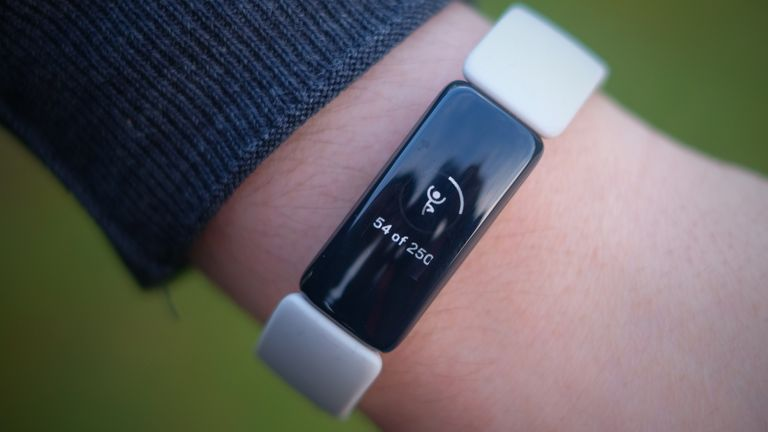
\includegraphics[width=0.66\textwidth]{figures/Fitbit inspire 2.jpg}
            \caption[Fitbit Inspire 2 colocada en una muñeca]
            {Fitbit Inspire 2 colocada en una muñeca. Imagen extraída de \cite{delves_fitbit_2022}}
            \label{figure:wearables:inspire_2}
        \end{figure}

        Los relojes inteligentes se pueden entender como una evolución de las pulseras de actividad en todos los sentidos. Visualmente, donde las pulseras incorporan una pequeña pantalla (en el caso de la Fitbit Inspire 2, de 0,72 pulgadas), relojes como el Samsung Galaxy Watch 6 (mostrado en la Figura \ref{figure:wearables:watch_6}) disponen de pantallas más grandes, siendo la de este reloj en específico de 1,5 pulgadas. 

        \begin{figure}[h]
            \centering
            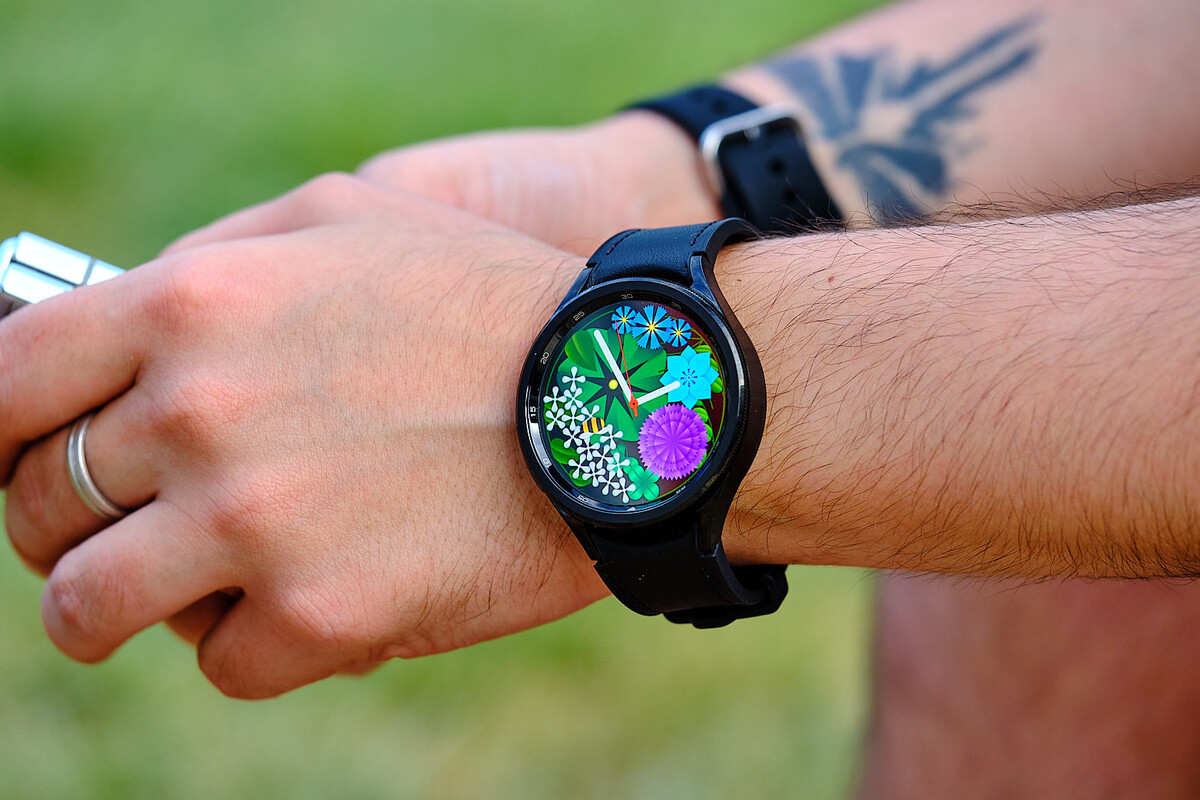
\includegraphics[width=0.66\textwidth]{figures/Samsung galaxy watch 6.jpeg}
            \caption[Samsung Galaxy Watch 6 colocado en una muñeca]
            {Samsung Galaxy Watch 6 colocado en una muñeca. Imagen extraída de \cite{alcolea_samsung_2023}}
            \label{figure:wearables:watch_6}
        \end{figure}

        En cuanto a las funciones relacionadas con la informática, toman las presentes en las pulseras como punto de inicio y añaden algunas más complejas, como la posibilidad de hacer pagos, responder a llamadas o de utilizar ciertas aplicaciones instaladas en el \gls{smartphone} (con limitaciones) \cite{alcolea_samsung_2023}. Lo mismo ocurre con las características de salud, incorporando funciones más avanzadas como el seguimiento de la presión arterial o del ciclo menstrual, la realización de \glspl{ecg}, o la medición de la temperatura corporal.

        Si bien estos son los dispositivos más comunes, en el mercado se pueden otros tipos de dispositivos \glspl{wearable} de naturaleza muy variopinta. Algunos de ellos son rastreadores como el AirTag de Apple, los cuales se pueden colocar en objetos para conocer/rastrear su ubicación en cualquier momento \cite{raspall_airtag_2024}; mientras que otros, como el Oura Ring, son anillos que permiten cierta monitorización física, similar a las de las pulseras de actividad \cite{garcia_oura_2021}.

        Por lo general, estos dispositivos se componen fundamental de un microprocesador, una batería y una serie de módulos hardware, tales como sensores o sistemas de comunicación inalámbrica \cite{luque_ordonez_dispositivos_2016}; los cuales permiten realizar las mediciones o interactuar con el exterior. Debido a las limitaciones de tamaño y especialmente de baterías de los dispositivos, normalmente suelen sincronizarse con un \gls{smartphone} la realización de ciertas tareas, o bien para procesar, almacenar o visualizar la información que recogen a través de aplicaciones específicas.

        Por último, cabe destacar no se trata de un mercado pequeño. Según datos del \textit{Worldwide Quarterly Wearable Device Tracker} \cite{international_data_corporation_worldwide_nodate}, el cual incluye como \glspl{wearable} a otros dispositivos como auriculares, el mercado de estos dispositivos tuvo un crecimiento interanual del 8,4\% en el segundo cuatrimestre de 2023, con una comercialización estimada de 520 millones de \glspl{wearable} durante todo el 2023 \cite{ricca_resurreccion_2023}.
        
    \subsection{Android}
        \label{section:contexto:Android}
        
        A grandes rasgos, Android es un Sistema Operativo orientado a dispositivos móviles basado en el núcleo Linux, diseñado para ser independiente de la arquitectura hardware de dichos dispositivos. Si bien fue planteado originalmente únicamente para teléfonos móviles, con el avance de la industria y el transcurso de las versiones ha adoptado un enfoque más amplio; siendo compatible con más dispositivos: tabletas, relojes inteligentes, televisores, pantallas de automóviles, etc. \footnote{No obstante, excepto en el caso de las tabletas, se trata de versiones \textbf{basadas} en Android con su propia 
        idiosincrasia y limitaciones.}
  
        Normalmente cuando se hace referencia a Android no se hace referencia únicamente al sistema operativo, sino a todo el ecosistema o plataforma creada entorno al mismo; como se hará a lo largo de este \gls{tfm}. Dicha plataforma o 
        \gls{framework} consta de numerosas capas, siendo el sistema operativo una parte de ellas, como se puede ver en la Figura \ref{figure:android:capas}. 

        \begin{figure}[h]
            \centering
            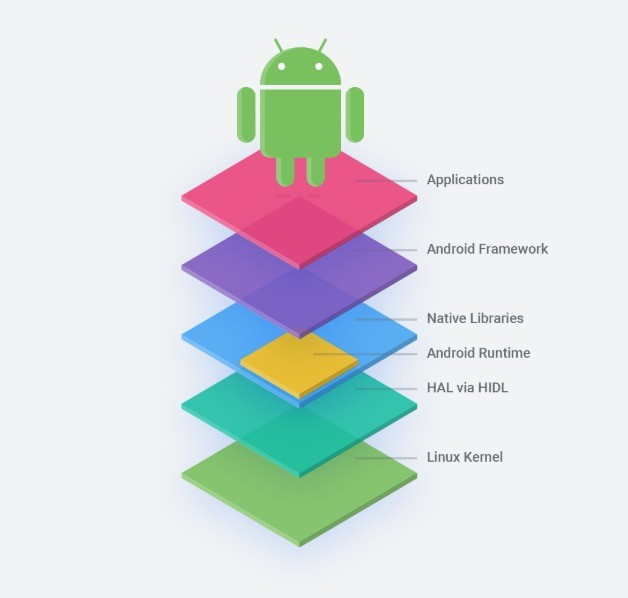
\includegraphics[width=0.66\textwidth]{figures/Android capas.jpg}
            \caption[Capas de Android]
            {Capas de Android. Imagen extraída de \cite{perez_aosp_2019}}
            \label{figure:android:capas}
        \end{figure}
        
        El sistema operativo como tal es denominado como \gls{aosp}, siendo su código fuente público. Cualquier persona puede acceder a él, descargarlo y modificarlo \cite{collado_que_2022}, pero en la inmensa mayoría de los terminales comercializados el sistema operativo es complementado con, entre otros, los \gls{gms}, servicios de Google que solo están disponibles bajo licencia; otorgada a los fabricantes que cumplen con una serie de requisitos. 

        Los \gls{gms} son utilizados para tareas como la gestión de notificaciones, servicios de geolocalización o para acceder a las herramientas de Google, tales como la tienda de aplicaciones Play Store. Asimismo, los fabricantes también pueden personalizar y añadir funciones al sistema operativo, lo que explica que dos terminales con la misma versión puedan verse tan diferentes entre sí. 
        
        Por otra parte, inicialmente Android fue desarrollado por la empresa homónima, si bien esta empresa fue comprada en 2005 por Google por 50 millones de dólares. La salida del sistema operativo se produciría dos años después, el 5 de noviembre de 2007, aunque el primer terminal que lo utilizaba (HTC Dream, también conocido como 
        T-Mobile G1) fue comercializado el 23 de septiembre de 2008 \cite{adeva_android_2023} \cite{marquez_asi_2022}; el cual se puede ver en la Figura \ref{figure:android:htc_dream}.

        \begin{figure}[h]
            \centering
            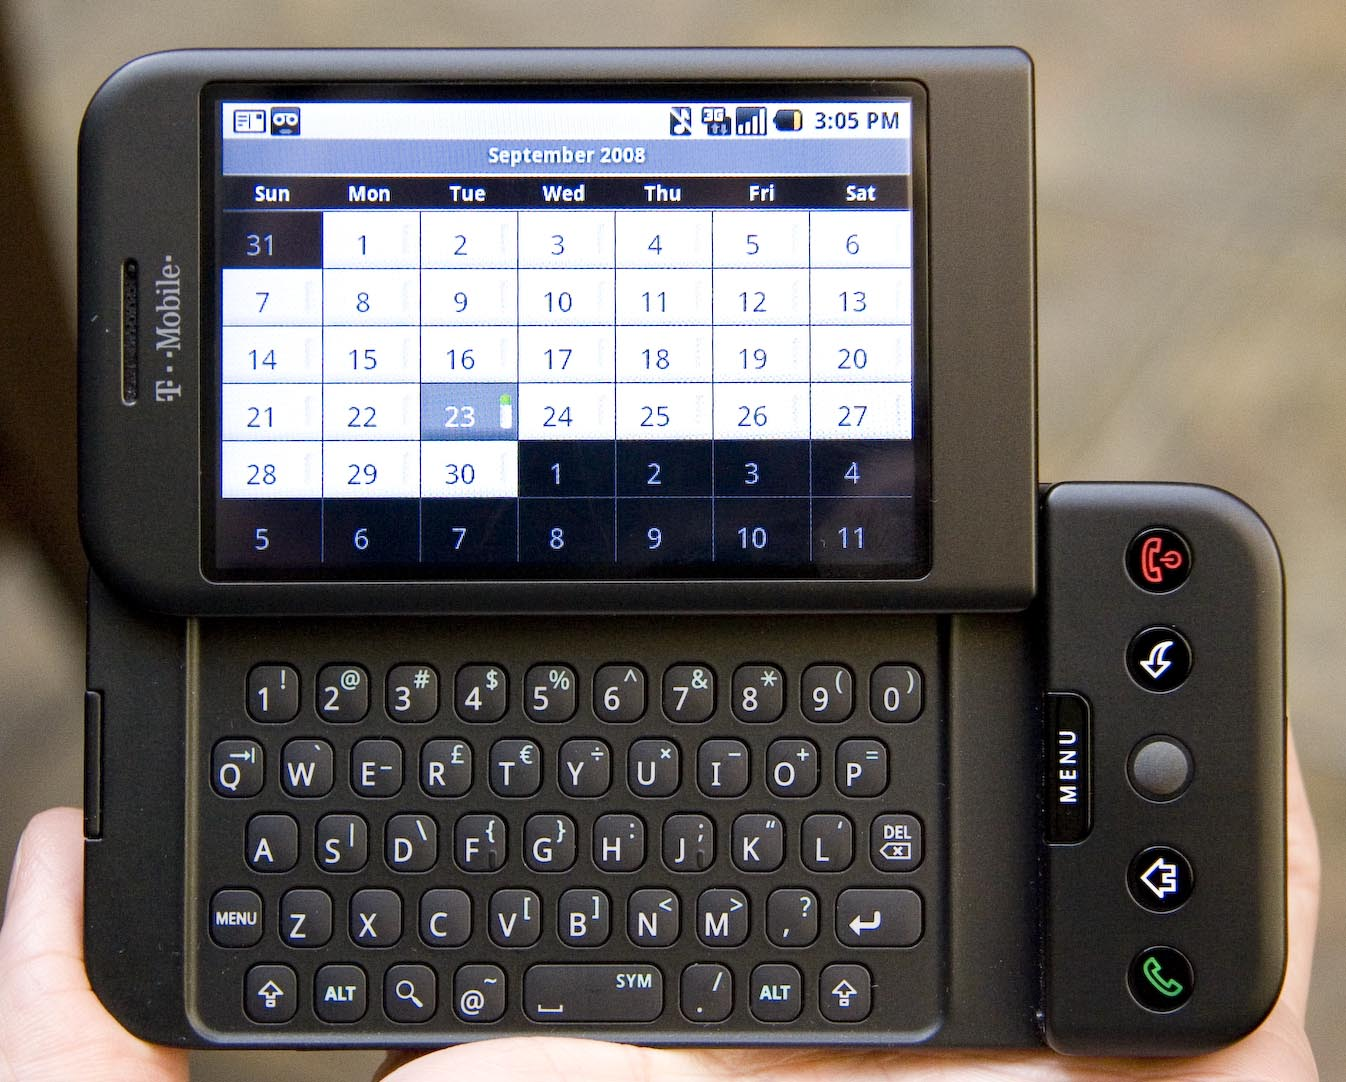
\includegraphics[width=0.5\textwidth]{figures/HTC Dream.jpg}
            \caption[HTC Dream en funcionamiento]{HTC Dream en funcionamiento. Imagen extraída de \cite{oryl_t-mobile_2008}}
            \label{figure:android:htc_dream}
        \end{figure}

        Desde entonces, numerosas versiones de Android han sido lanzadas, siendo la última versión estable a fecha de realización de este documento Android 14; estableciéndose por parte de Google la \textit{costumbre} de lanzar cada año una nueva versión principal. En cada una de ellas se introducen nuevas características, pero esto no significa que todos los dispositivos puedan actualizarse a la última. 
        
        Los fabricantes no están obligados a actualizar sus terminales, lo que en la práctica supone que las nuevas versiones no son utilizadas masivamente y que los programadores deben de tener en cuenta las versiones antiguas en sus aplicaciones. No obstante, a lo largo del último año, actores como la propia Google \cite{ricca_google_2023} y Samsung \cite{ramirez_samsung_2024} se han comprometido a proporcionar siete años de actualizaciones para algunos de sus nuevos dispositivos.
        
        Debido a que Google dejó de publicar oficialmente las estadísticas de uso de su sistema operativo, no es posible conocer con plena exactitud dichas cifras. La comunidad se ha encargado de estimar dicha información \cite{belinski_android_nodate}; relevando que a fecha de abril de 2024 sólo el 16,3\% de los dispositivos tienen la última versión, mientras que las versiones 13, 12 y 11 están presentes en el 26,2\%, 17\% y 16,2\%, respectivamente; permaneciendo el 24,3\% con versiones lanzadas previamente al año 2020.

        \begin{figure}[h]
            \centering
            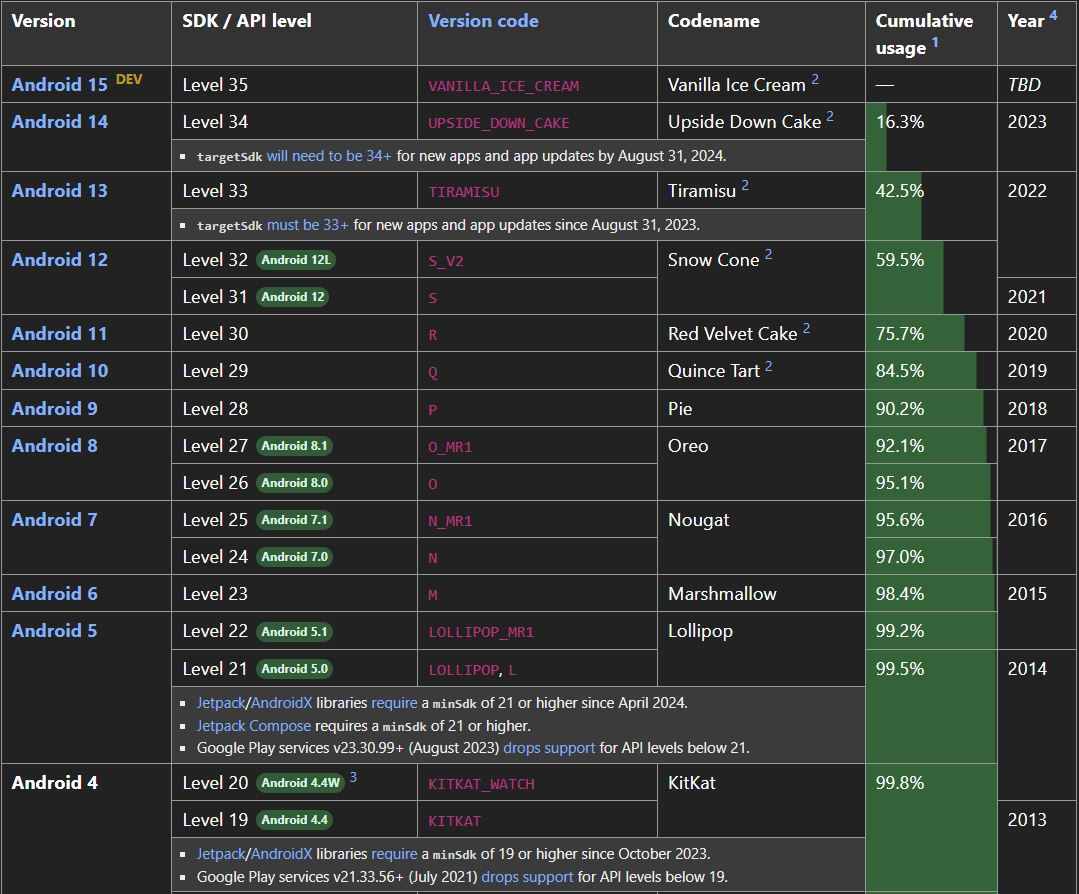
\includegraphics[width=0.8\textwidth]{figures/Android usage.JPG}
            \caption[Estadísticas acumulativas de las versiones de Android]
            {Estadísticas acumulativas de las versiones de Android. Imagen extraída de \cite{belinski_android_nodate}}
            \label{figure:android:usage}
        \end{figure}

        Por último, a fecha de junio de 2024, Android dispone de una cuota de mercado del 72,15\% en el segmento de sistemas operativos para dispositivos móviles, teniendo su mayor rival, el sistema operativo iOS (propiedad de Apple) un 27,19\% \cite{melo_infografi_2024}. Entre ambos acaparan el mercado, con un 99,34\% de cuota de mercado. En cuanto a España, según la \gls{cnmc} en una encuesta realizada en el segundo trimestre de 2023 a 9.095 individuos, la cuota de mercado Android es del 78,73\% por el 16,3 de iOS \cite{comision_nacional_de_los_mercados_y_la_competencia_android_2023}.

    \subsection{Kotlin}

        Kotlin es un lenguaje de programación desarrollado por JetBrains\footnote{JetBrains es una empresa muy reconocida dentro de la industria por crear una serie de entornos de desarrollo muy populares, como PHPStorm, CLion o Intellij IDEA. Sobre este último está construido Android Studio, el entorno de desarrollo oficial dentro de Android.} y publicada su primera versión estable el 15 de febrero de 2016. El objetivo de este lenguaje, basado en Java, fue tan sencillo como ambicioso: crear un lenguaje conciso (permitiendo reducir la cantidad de código \gls{boilerplate}), con soporte de nuevas funcionalidades; pero sin renunciar a la rapidez de compilación de Java ni al todo el código escrito en él \cite{rao_k_history_nodate}. 

        Sus principales características son las siguientes \cite{kotlin_help_kotlin_nodate} \cite{android_developers_enfoque_nodate}:
        \begin{itemize}
            \item Interoperable en ambos al 100\% con Java, lo que facilita la reutilización de código ya existente.
            \item Permite escribir código más seguro, al resolverse en el diseño del lenguaje problemas crónicos de Java como las \textit{Null Pointer Exception}. Según datos internos de Google, las aplicaciones escritas en Kotlin tienen un 20\% de probabilidades menos de fallar \cite{android_developers_enfoque_nodate}.
            \item Soporte nativo y estructurado para la programación concurrente y asíncrona mediante construcciones como las corrutinas y los flujos.
            \item Desarrollo multiplataforma, no solo para Android: aplicaciones web, \textit{backend} e iOS.
            \item Permite desarrollos en varios paradigmas: orientada a objetos, funcional, imperativa, etc.
        \end{itemize}

        Cabe resaltar que durante el diseño de Android se estableció que el lenguaje principal para desarrollar aplicaciones sería Java, si bien incorpora soporte para utilizar código C y C++ \cite{android_developers_como_nodate}. No
        obstante, al ser Java un lenguaje interpretado sobre la \gls{jvm}, cabía la posibilidad de soportar otros lenguajes que también utilizasen la \gls{jvm}.
        
        En la conferencia de Google \textit{I/O} de 2017, fue anunciado el soporte oficial y completo de Kotlin dentro de Android, para en 2019 convertirse en el lenguaje de referencia para el desarrollo de Android \cite{braun_celebrating_2022}, por lo que los desarrollos de librerías y herramientas relacionadas con Android están escritas en este lenguaje, aprovechando al máximo sus nuevas características. 
        
        Por tanto, si bien es interoperable con Java, se recomienda que los nuevos desarrollos lo utilicen \cite{lardinois_kotlin_2019}, como se ha realizado en este \gls{tfm}. Por último, según \cite{kotlin_help_kotlin_nodate}, aproximadamente el 95\% del top mil de aplicaciones Android usan en alguna medida Kotlin, por lo que su uso está plenamente justificado.
        
    \subsection{Salud Conectada}
        \label{section:salud_conectada}
        En la conferencia \textit{I/O}, de 2022 se anunció \textit{Health Connect} (o \textit{Salud Conectada} en castellano\footnote{A lo largo de este \gls{tfm} se utilizarán indistintamente los términos \textit{Health Connect} y \textit{Salud Conectada}.}), una plataforma creado por Google junto con Samsung \cite{wilk_introducing_2022} que aglutina todos los datos relacionados con salud dentro del ecosistema Android. 
        
        Este componente, lanzado en fase beta en noviembre de 2022, se puede encontrar preinstalado en algunos dispositivos Android a partir de la versión 14 \cite{ayuda_de_android_informacion_nodate} o como una aplicación para dispositivos Android 9 o superior \cite{pandey_health_2023} \footnote{Cabe destacar que esta aplicación es parte de los \gls{gms} y no del sistema operativo propiamente dicho o \gls{aosp}.}. A fecha de mayo de 2023, se estima que más de 100 aplicaciones han integrado \textit{Salud Conectada}, incluyendo las aplicaciones de las pulseras Fitbit y Samsung, Peloton o Oura, entre otros \cite{malik_googles_2023}.
        
        Esta herramienta proporciona una solución a una problemática muy relevante en el ámbito de los \glspl{wearable}. Como se describió en la Sección \ref{section:contexto:wearables}, los fabricantes procesan, almacenan y visualizan los datos recogidos en su aplicación; radicando el problema en el nulo reaprovechamiento de estos datos. La posición casi unánime dentro la 
        industria hasta la aparición de este componente se basaba en aislar estos datos  dentro de su ecosistema \cite{ramirez_android_2022} \cite{rahman_android_2023}. 
        
        Por tanto, para utilizar dichos datos en otras aplicaciones las posibilidades residían en el uso de a sistemas propietarios como \textit{Google Fit}, cuyos datos se almacenaban en la nube, o a través de proyectos \gls{open-source} como \textit{Gadget Bridge}, que acceden a datos mediante ingeniería inversa \cite{freeyourgadget_gadgetbridge_nodate}. Estas opciones plantean claras desventajas, como desde los potenciales problemas de privacidad en el caso de \textit{Google Fit}; hasta cuestiones legales y dificultad de compatibilidad y uso en el caso de \textit{Gadget Bridge}.
        
        Como se visualiza en la Figura \ref{figure:health_connect:arquitectura} \textit{Salud Conectada} consta de varias capas. Para los usuarios finales se presenta mediante una aplicación, que entre otras cuestiones permite ver a los usuarios los datos recogidos por tipo de dato, o los accesos a sus datos; como recoge la Figura \ref{figure:health_connect:ejemplo}. Para los desarrolladores se muestra como un sistema de acceso a los datos, el cual define una serie de permisos y un acceso a través de una \gls{api}.

        \begin{figure}[h]
            \centering
            \includegraphics[width=0.33\textwidth]{figures/Arquitectura básica de Health Connect.png}
            \caption[Arquitectura básica de \textit{Salud Conectada}]
            {Arquitectura básica de \textit{Salud Conectada}. Imagen extraída de \cite{wilk_introducing_2022}.}
            \label{figure:health_connect:arquitectura}
        \end{figure}

        \begin{figure}[h]
            \begin{subfigure}[b]{0.49\textwidth}
                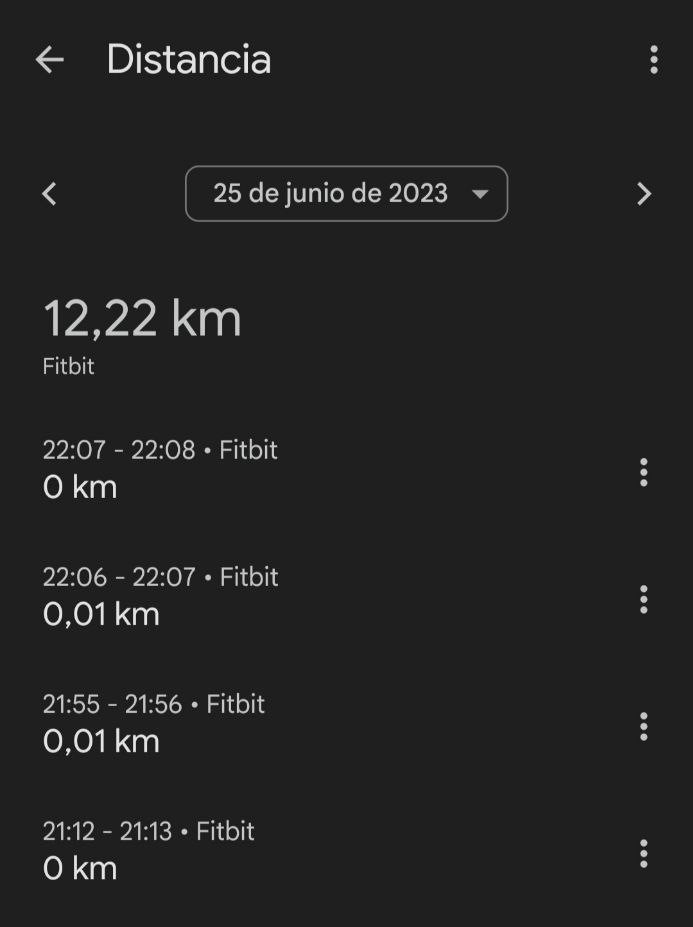
\includegraphics[width=1\linewidth]{figures/Health Connect lectura datos.jpg}
            \end{subfigure}
            \hfill
            \begin{subfigure}[b]{0.49\textwidth}
                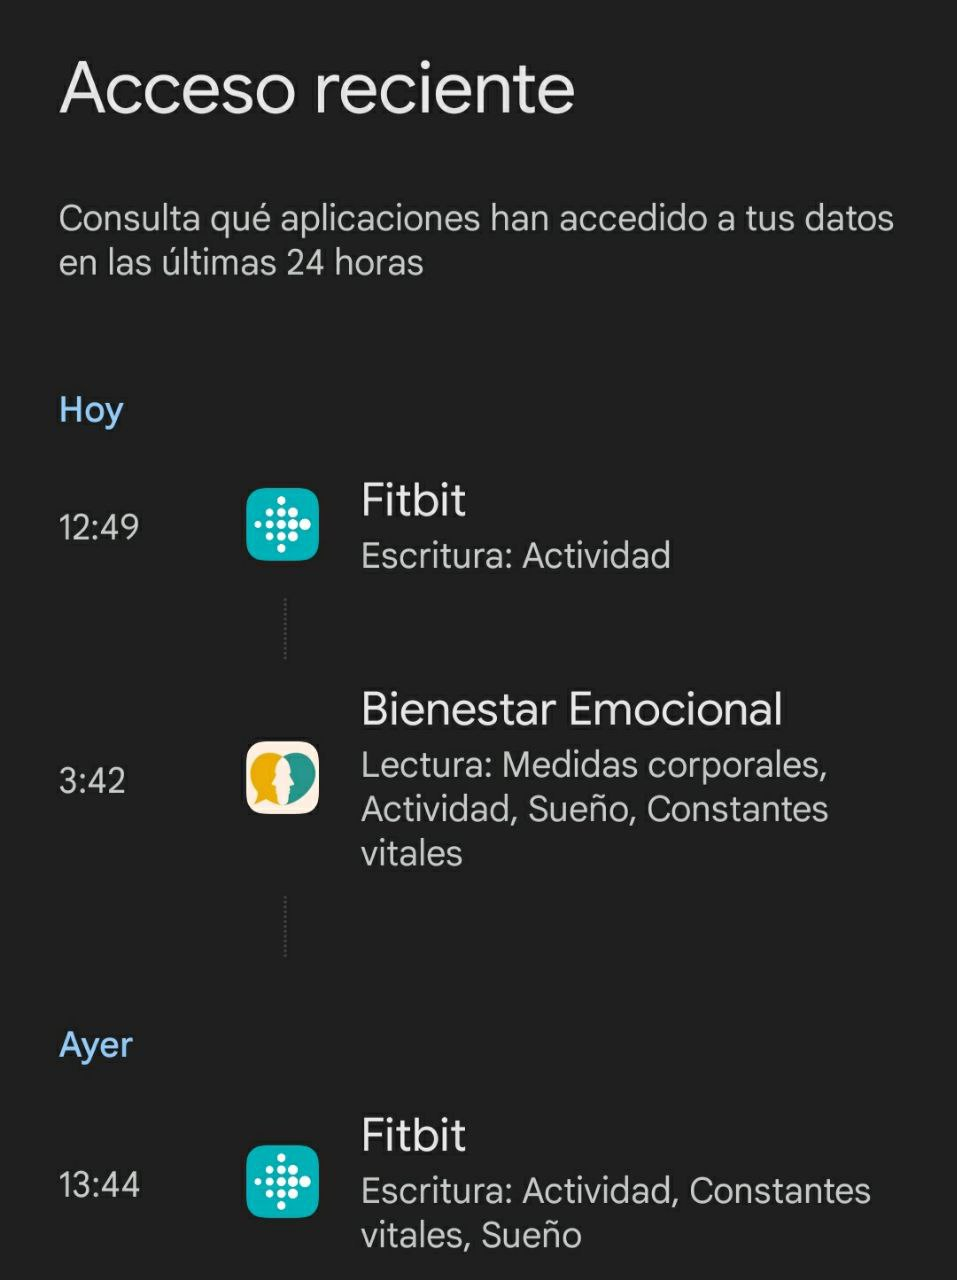
\includegraphics[width=1\linewidth]{figures/Health Connect acceso reciente.jpg}
            \end{subfigure}
            \caption{Ejemplo de algunas de las funciones de \textit{Salud Conectada} para los usuarios, como la visualización de datos o el acceso de aplicaciones a datos}
            \label{figure:health_connect:ejemplo}
        \end{figure}
        
        La plataforma puede gestionar datos como la actividad física, el sueño, la nutrición o incluso el ciclo menstrual\footnote{La lista completa de los datos que puede registrar \textit{Salud Conectada} se encuentra 
        disponible en \cite{android_developers_lista_nodate}}, siendo un intermediario entre las aplicaciones que generan o escriben dichos datos y las que quieren acceder a esos datos. 
        
        Por tanto, esta \gls{api} estandariza el acceso a todas las fuentes de datos, independientemente de su procedencia; lo que simplifica enormemente tanto la lectura como escritura de los datos. Además, el sistema permite consultar
        datos agregados, pudiendo ser una agregación acumulativa (como el total de distancia caminada en un intervalo de tiempo) o estadística (las pulsaciones mínimas, máximas o promedio en un intervalo de tiempo).

        Por otra parte, este sistema rompe con el esquema de \textit{Google Fit}, almancenándose los datos localmente. Además, el acceso a los mismos esta fuertemente granularizado; estando en manos del usuario la decisión de qué aplicaciones tienen acceso (tanto lectura como escritura) a cada tipo de registro \cite{saez_google_2022}, como muestra la Figura \ref{figure:health_connect:granularidad_permisos}. 

        \begin{figure}[h]
            \centering
            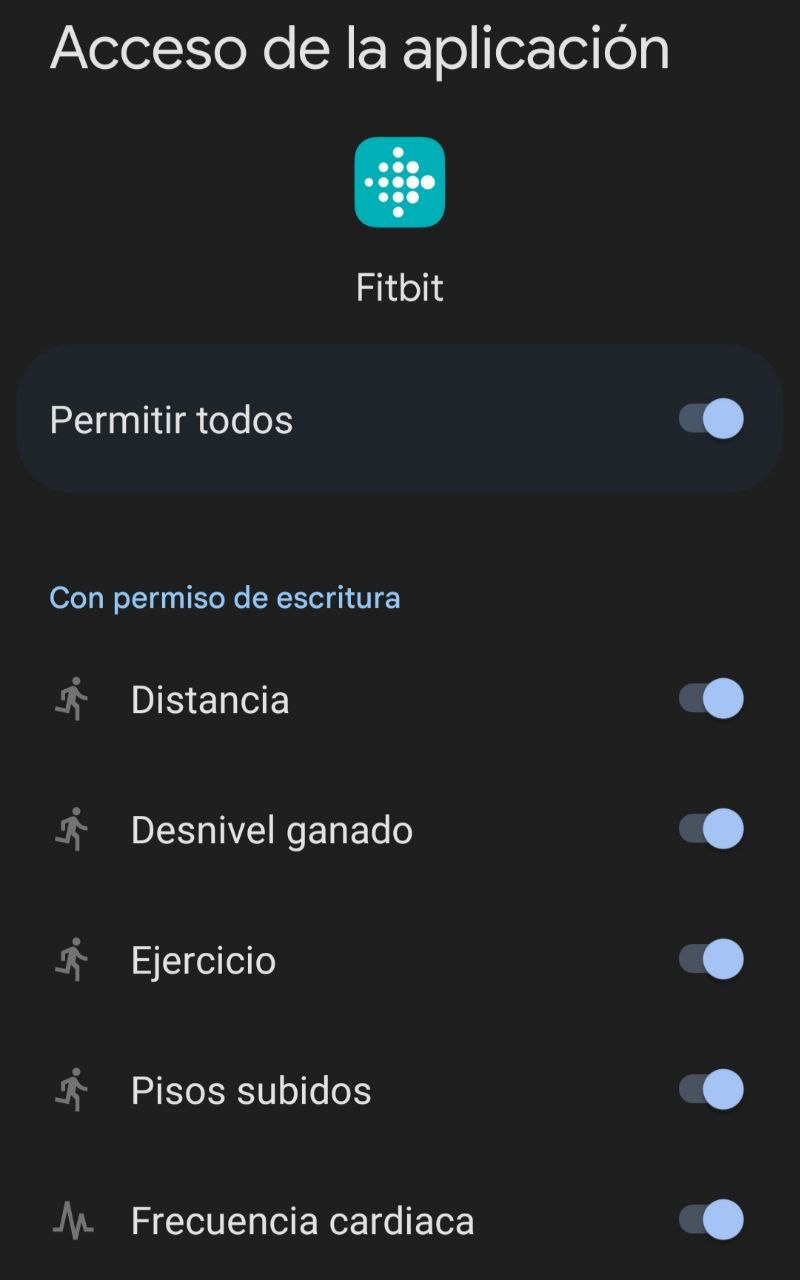
\includegraphics[width=0.5\textwidth]{figures/Health connect permisos fitbit.jpg}
            \caption[Granularidad de los permisos de \textit{Salud Conectada}]
            {Granularidad de los permisos de \textit{Salud Conectada}.}
            \label{figure:health_connect:granularidad_permisos}
        \end{figure}

        
        Asimismo, las aplicaciones solo pueden leer datos con una antigüedad de hasta 30 días previos a su instalación \cite{android_developers_preguntas_nodate}, registrándose (como se pudo ver en la Figura \ref{figure:health_connect:ejemplo}) todas las lecturas y escrituras en el sistema.

        En definitiva, si bien está aún en desarrollo y en vías de convertirse en estándar dentro de Android, esta plataforma permite a los desarrolladores la abstracción completa del hardware de recolección de datos biométricos, lo que permite reducir notablemente los costes de desarrollo de nuevos productos, permitiendo además un mayor control al usuario de sus datos sensibles, mejorando la transparencia de las aplicaciones.

    \subsection{Jetpack Compose}

        \textit{Jetpack Compose} es un \gls{sdk} de Android para el desarrollo de interfaces gráficas, lanzado en su primera versión estable el 28 de julio de 2021 por Google \cite{bellini_jetpack_2021}. Asimismo, Jetpack Compose es parte de un \gls{sdk} más grande conocido como \textit{Android Jetpack}, el cual es promovido por Google para mejorar el desarrollo dentro de Android \cite{huaman_que_2018} \cite{android_developers_recursos_nodate}. 
        
        \textit{Jetpack Compose} permite desarrollar en el ecosistema Android de forma nativa interfaces gráficas de manera declarativa como en los sistemas React, Flutter o SwiftUI; siguiendo las tendencias actuales de la industria en el desarrollo de aplicaciones móviles. 

        Hasta la aparición de esta herramienta, el desarrollo interfaces gráficas nativas en Android se realizaba con el enfoque conocido como programación imperativa. En este tipo de desarrollo es necesario especificar exhaustivamente cómo se va a construir dicha interfaz gráfica. En dicho proceso (conocido en Android como sistema de vistas) se codificaba un fichero \gls{xml}, en el que se describían todos los elementos gráficos (botones, textos, etc.); para que la aplicación accediera a dichos elementos y le aplicara manualmente modificaciones y transformaciones \cite{deloitte_spain_programacion_2021}. 

        En cambio, el enfoque declarativo permite describir cómo se desea que sea la interfaz gráfica. Las interfaces que se construyen mediante \textit{Jetpack Compose} pueden estar interconectadas a estados descritos por el programador, describiendo cómo es la interfaz para cada posible estado. Cuando dicho estado cambia, el sistema cambia automáticamente la interfaz gráfica mostrada, simplificando y reduciendo enormemente el proceso de desarrollo \cite{leiva_que_2021}. 

        A diferencia del sistema anterior, los componentes gráficos están desacoplados 
        del sistema operativo; por lo que ya no se depende de la versión del terminal para mostrar correctamente la interfaz gráfica. Como se vió en la Sección 
        \ref{section:contexto:Android}. la fragmentación en Android es un 
        problema endémico, lo que complicaba notablemente el diseño de las aplicaciones Asimismo, es compatible con los componentes \gls{xml} del sistema anterior, lo que facilita la migración de los proyectos antiguos a este nuevo paradigma. 

        No obstante, está diseñado para ser utilizado casi exclusivamente desde Kotlin, por lo que en algunos casos puede resultar en un pico de dificultad relevante si el equipo de desarrolladores no domina el lenguaje.
    
    \subsection{Material Design 3}
        \textit{Material Design 3} (también conocido como \textit{Material You}) es la tercera iteración del conjunto de principios y directrices de diseño de Google, como respuesta a la creciente ubiquidad de Android: móviles con pantallas plegables, \textit{smartwatch}, televisores \cite{ramirez_que_2022}, etc. Su primera implementación estable para \textit{Jetpack Compose} fue lanzada el 24 de octubre de 2022 \cite{singh_material_2022}.
        
        Al ser utilizado por Google para la creación de elementos gráficos tanto en sus aplicaciones como en el sistema operativo, se convirtió en la guía de diseño \textit{de facto} dentro del ecosistema Android.

        Sus principales características son las siguientes \cite{material_design_material_nodate}:
        \begin{itemize}
            \item Apuesta por la personalización de la interfaz gráfica: los diseñadores pueden elaborar su paleta de colores mediante la herramienta 
            \textit{Material Design Builder} \cite{material_design_material_nodate-1} (mostrada en la Figura \ref{figure:material_design_3:builder}), la cual garantiza el cumplimiento de la guía de accesibilidad \gls{wcag} 2.0 del consorcio \gls{w3c} \cite{w3c_web_2008}. Para ello se pueden definir hasta tres colores principales, los cuales serán utilizados para los elementos gráficos de forma totalmente transparente al programador.

                \begin{figure}[h]
                    \centering
                    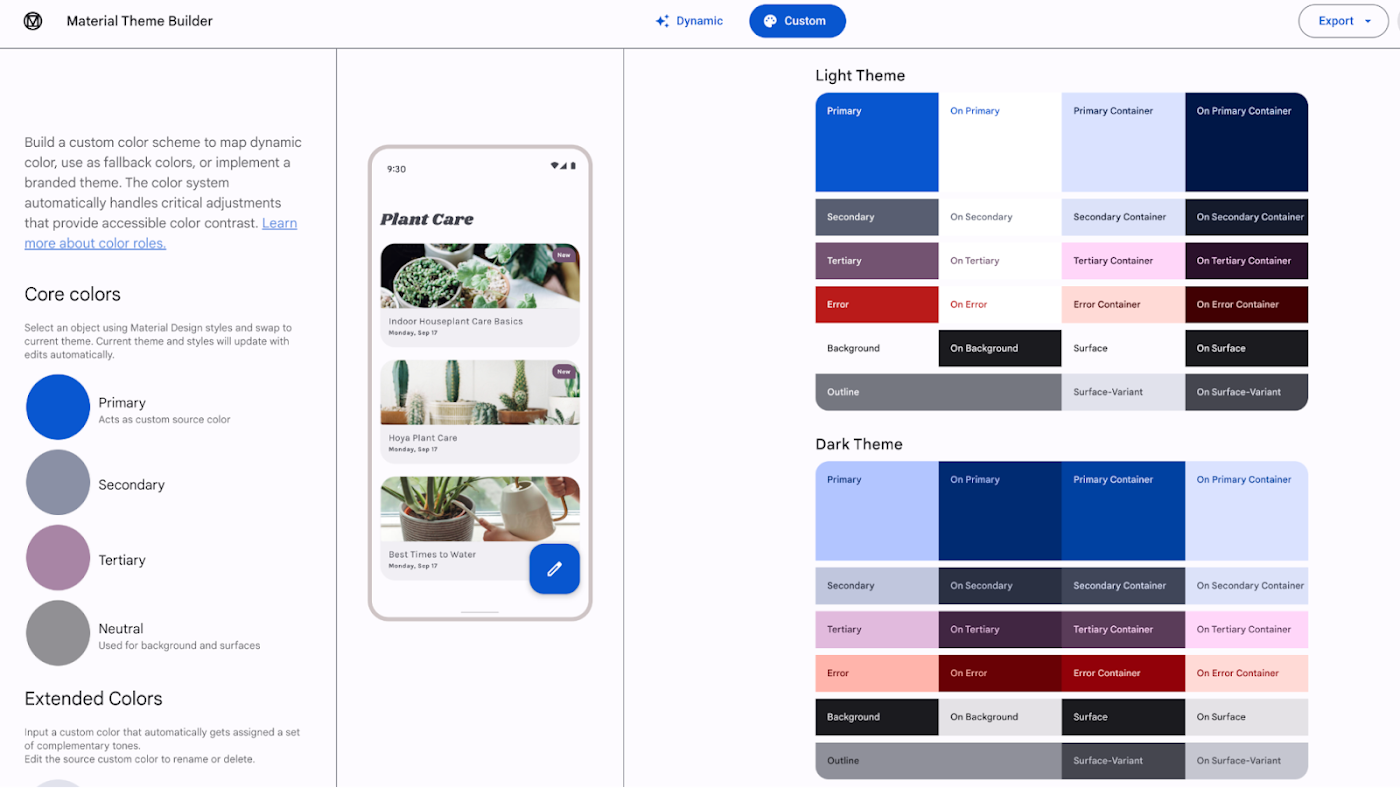
\includegraphics[width=0.85\textwidth]{figures/Material Design Builder example.png}
                    \caption[Ejemplo de uso de la herramienta \textit{Material Design Builder}]
                    {Ejemplo de uso de la herramienta \textit{Material Design Builder}. Imagen extraída de \cite{singh_material_2022}.}
                    \label{figure:material_design_3:builder}
                \end{figure}

            Además, si el dispositivo dispone de Android 12 o superior, pueden tomarse dichos colores desde el fondo de pantalla del usuario, incrementando exponencialmente la personalización; si bien se permite establecer colores \textit{fijos} para ciertos contenidos.
            \item Soporte nativo para categorizar el tamaño de la pantalla del dispositivo, tanto en altura como en anchura, como se muestra en las Figuras \ref{figure:material_design_3:height_classes} y \ref{figure:material_design_3:width_classes} respectivamente.

                \begin{figure}[h]
                    \centering
                    \includegraphics[width=0.85\textwidth]{figures/Categorías de ventana según altura.png}
                    \caption[Categorías de pantalla según altura]
                    {Categorías de pantalla según altura. Imagen extraída de \cite{android_developers_window_nodate}}
                    \label{figure:material_design_3:height_classes}
                \end{figure}
                
                \begin{figure}[h]
                    \centering
                    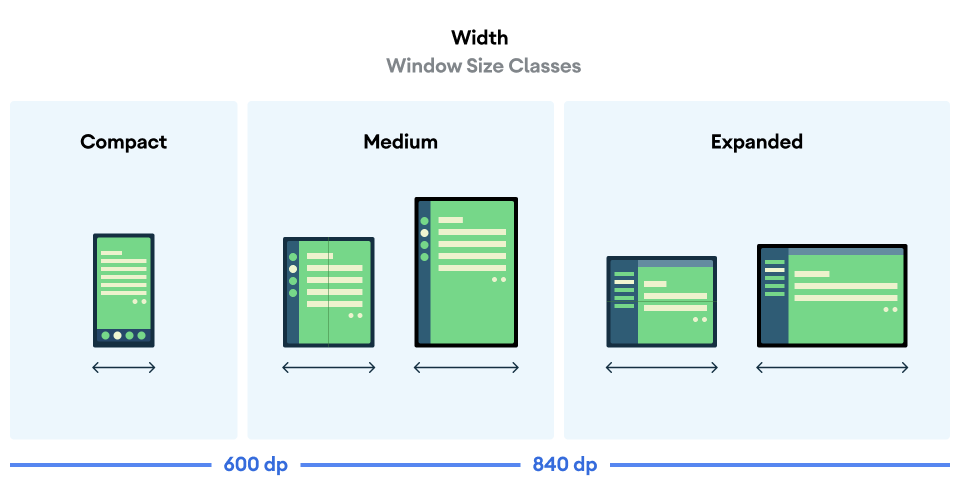
\includegraphics[width=0.85\textwidth]{figures/Categorías de ventana según anchura.png}
                    \caption[Categorías de pantalla según anchura]
                    {Categorías de pantalla según anchura. Imagen extraída de \cite{android_developers_window_nodate}}
                    \label{figure:material_design_3:width_classes}
                \end{figure}

            \item Sistema de fuentes basado en estilos principales para cada tipo de contenido: desde titulares hasta etiquetas, pasando por títulos, cuerpos de texto, etc.
            \item Soporte nativo para animaciones, las cuales ya son utilizadas en los componentes gráficos nativos, como los \textit{switch}.
            \item Evolución de muchos elementos gráficos, como las tarjetas, botones, selectores de fechas, etc. La Figura \ref{figure:material_design_3:elementos_graficos} muestra algunos de estos elementos.
                \begin{figure}[h]
                    \centering
                    \includegraphics[width=0.75\textwidth]{figures/Elementos gráficos material design 3.png}
                    \caption[Algunos elementos gráficos de \textit{Material Design 3}]
                    {Algunos elementos gráficos de \textit{Material Design 3}. Imagen extraída de \cite{cerda_material_2022}}
                    \label{figure:material_design_3:elementos_graficos}
                \end{figure}
            \item Sistema de formas o \textit{redondeo} multinivel para modernizar los elementos gráficos y hacerlos más distinguibles entre sí.
            \item Mejoras en el concepto conocido como \textit{elevación}, basándose en colores y no en sombras. Este elemento permite superponer elementos y transmitir gráfica y visualmente la importancia de cada uno de ellos.
            \item Soporte nativo para tema claro y oscuro, resolviendo la ausencia de dicho soporte.
        \end{itemize}

        Se trata en definitiva de una modernización del lenguaje de diseño, haciéndolo más 
        atractivo y completo a la vez que se garantiza cierta accesibilidad para los usuarios. Se han alejado de lo puramente funcional para abrazar el mundo de la personalización para el usuario.

    \subsection{Room}
        Uno de los servicios que provee Android es SQLite, un \gls{sgbd} relacionales de bajo nivel, destinado para ser utilizado por las aplicaciones finales. No obstante, para muchas de ellas es un modelo demasiado rígido, por lo que Google creó en 2017 esta librería, la cual hace de intermediario entre SQLite y las aplicaciones \cite{leiva_room_2020}. 
        
        Técnicamente hablando se trata de una capa de abstracción sobre dicho sistema gestor, la cual permite reducir la complejidad de los usos comunes de la base de datos; sin perder el acceso a SQLite. Asimismo, esta librería brinda otras ventajas, como la verificación de las consultas
        \gls{sql} en tiempo de compilación \cite{android_developers_como_nodate}.

        Los elementos básicos para utilizar esta librería son los siguientes:
        \begin{itemize}
            \item \gls{dao}. En este elemento se crean todas las operaciones que se realizan sobre la base de datos: consultas, inserciones, etc.
            \item Entidades, las cuales se corresponden con una clase en Kotlin y normalmente con una tabla de base de datos. Con esta estructura se crean las tablas bases de datos, realizándose un mapeo de dichas tablas a objetos. Sobre los atributos de los objetos se pueden realizar anotaciones para establecer claves, índices, etc.
            \item Clase base de datos, donde se especificarán las entidades de la propia base de datos y cómo se instancia, reduciendo el código \gls{boilerplate}. Este procedimiento se detalla mediante una función que configura ciertos parámetros, como el nombre del fichero de la base de datos o características extra, como el uso de cifrado. Para la construcción de dicha instancia Room implementa el patrón factoría.
        \end{itemize}
    
    \subsection{Work Manager}
        \textit{Work Manager} es el componente oficial de Android para la planificación de subtareas, diseñada para simplificar el uso del amalgama de librerías para esta
        funcionalidad presentes en Android. Hasta entonces, según la versión del sistema, debían utilizarse unas u otras, estableciendo \textit{Work Manager} una única interfaz para esta funcionalidad; encargándose internamente de utilizar la librería correcta a bajo nivel \cite{android_developers_workmanager_nodate}.
        
        Este componente admite dos tipos de tareas: puntuales y periódicas; las cuales se pueden planificar o cancelar. Además de la planificación temporal, permite el establecimiento de algunas restricciones, como que el dispositivo esté cargándose o disponga de conexión a internet, ejecutándose la tarea en cuestión solo cuando se cumplan todas las restricciones y directrices \cite{android_developers_arquitectura_nodate}.

        Asimismo, permite establecer una política de reintentos si las tareas no se han ejecutado correctamente, por lo que es la solución recomendada para los casos de uso que necesiten realizar ciertas operaciones de manera fiable.

    \subsection{Lottie}
        \textit{Lottie} es una biblioteca creada por Airbnb, la cual que busca facilitar la creación y uso de animaciones en entornos multiplataforma (web, iOS, Android, entre otros) \cite{rubianes_lottie_2021}. A diferencia de archivos como los \gls{gif}, esta librería permite que las animaciones puedan escalarse sin perder calidad (como en los ficheros \gls{svg}), haciendo hincapié en el rendimiento.

        Concretamente, la librería renderiza en tiempo real animaciones de \textit{Adobe After Effects}, las cuales son exportadas como ficheros \gls{json} que serializan dicha animación \cite{airbnb_design_lottie_nodate}, utilizando una extensión \gls{open-source} conocida como \textit{Bodymovin}. Por tanto, estas animaciones pueden ser personalizadas completamente, a la vez que se reducen las necesidades de cómputo para mostrarlas. 
        
        \begin{figure}[h]
            \centering
            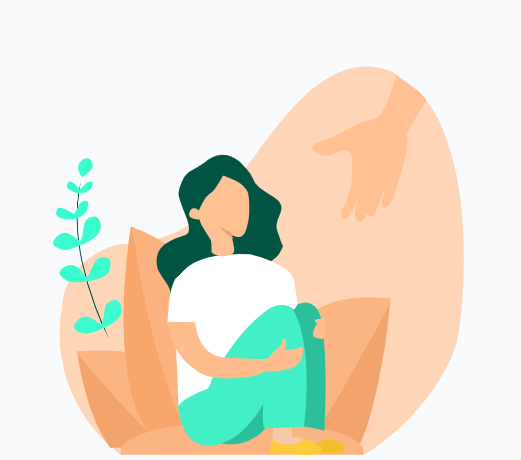
\includegraphics[width=0.5\textwidth]{figures/Animacion de ejemplo.PNG}
            \caption{Vista previa de una animación personalizada}
            \label{figure:lottie:animacion_ejemplo}
        \end{figure}

        En este \gls{tfm} será abordada únicamente la personalización de animaciones gratuitas aportadas por la comunidad y su presentación en la aplicación; y no la creación de nuevas. Para conseguir dichas animaciones se ha utilizado el portal \href{https://lottiefiles.com/}{LottieFiles}.

    \subsection{Vico}
        
        Vico es una biblioteca \gls{open-source} para la realización de gráficos, creada por Patryk Goworowski. Su particularidad reside en su compatibilidad tanto con el sistema de vistas tradicional como con \textit{Jetpack Compose}, algo único en el ecosistema de Android \cite{goworowski_vico_nodate}. Si bien no es tan potente como otras librerías como \textit{MPAndroid}, sus posibilidades son más que suficientes para este \gls{tfm}. 
        
        Gracias al soporte nativo de \textit{Jetpack Compose} y \textit{Material Design 3}, esta librería introduce algunas mejoras en las gráficas, como una interconexión directa con los colores que se utilizan en tiempo de ejecución, incrementando la coherencia visual de la aplicación.

        Vico permite crear únicamente gráficos de barras y de líneas, ejemplificadas en las Figuras \ref{figure:vico:ejemplo_barras} y \ref{figure:vico:ejemplo_lineas}, respectivamente. Su humilde enfoque, si bien puede condicionar y limitar notablemente su uso, permite que contenga numerosos añadidos completamente personalizables, tales como: leyendas, marcadores (tanto fijos como temporales), \textit{líneas umbral}, personalización de los ejes, etc.

        \begin{figure}[h]
            \centering
            \includegraphics[width=0.55\textwidth]{figures/Gráfica de barras con vico.jpg}
            \caption{Ejemplo de gráfica de barras realizada con Vico}
            \label{figure:vico:ejemplo_barras}
        \end{figure}

        \begin{figure}[h]
            \centering
            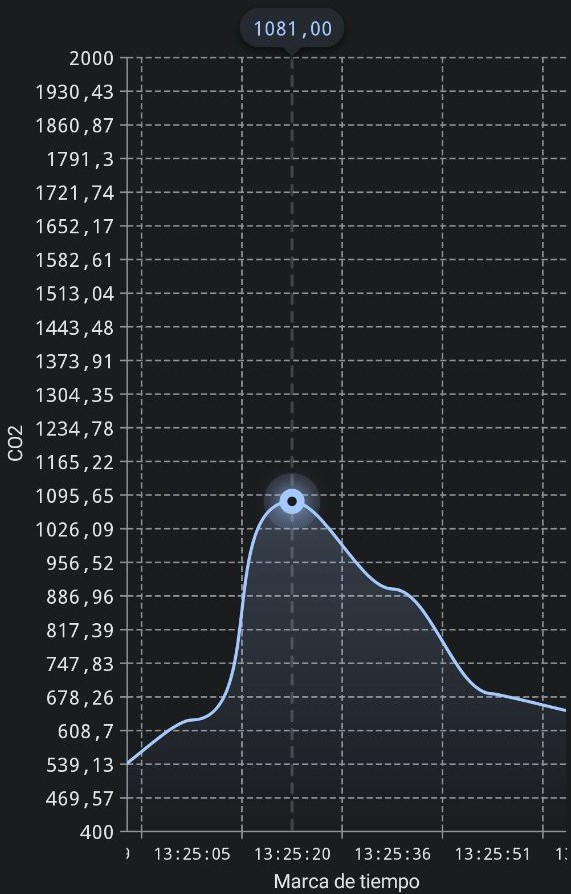
\includegraphics[width=0.4\textwidth]{figures/Gráfica de líneas con vico.jpg}
            \caption{Ejemplo de gráfica de líneas realizada con Vico}
            \label{figure:vico:ejemplo_lineas}
        \end{figure}
        
        
        Asimismo, su mantenimiento y mejora es notable y constante. Nuevas versiones son lanzadas cada pocas semanas \cite{goworowski_vico_2023-1}, mientras que el soporte ofrecido en su repositorio es rápido y detallado \cite{goworowski_vico_2023}. Además, dispone de numerosa documentación para aprender a utilizarla rápidamente, si bien no cubre los casos de uso más avanzados. Por último, dispone de una aplicación de demostración que permite ver rápidamente las posibilidades que ofrece la librería.

    \subsection{Python}
        Python es un lenguaje de programación interpretado creado por Guido Van Rossum en 1991, con un marcado enfoque de construir código de la manera más clara y legible posible. Es uno de los lenguajes más populares de la escena, gracias a su facilidad de uso y a su enorme comunidad de desarrolladores. Estos últimos han creado un enorme ecosistema de librerías que facilita la creación de nuevos proyectos, especialmente para prototipos.

        Actualmente es utilizado para todo tipo de tareas, tales como desarrollo web, aplicaciones científicas, inteligencia artificial o análisis de datos; casi siempre apoyándose en potentes librerías que mejoran notablemente el propio lenguaje. 

        Sus principales características son las siguientes:
        \begin{itemize}
            \item Soporte mutiparadigma: como Kotlin, se puede utilizar programación imperativa, orientada a objetos o funcional en cualquier momento.
            \item Gran biblioteca estándar, la cual facilita muchas operaciones mundanas, como la lectura de archivos \gls{json}.
            \item Soporte multiplataforma, gracias a la compatibilidad de su intérprete con todos los sistemas operativos principales. Llega hasta tal punto que un subconjunto del lenguaje (\textit{MicroPython}) es compatible con algunos microcontroladores.
            \item Sistema de tipos fuertemente tipado y dinámico, lo que permite que una variable pueda cambiar de tipo fácilmente.
            \item Facilidad de instalación de librerías gracias a la herramienta pip.
        \end{itemize}
    
    \subsection{Flask}

        \textit{Flask} es un popular entorno ligero o \gls{microframework} de Python utilizado para construir aplicaciones web, tanto como páginas como \gls{api}. Diseñado para ser ligero y fácil de usar, \textit{Flask} proporciona las herramientas necesarias para crear dichas aplicaciones web de una manera minimalista, rápida y eficiente, en sintonía con la propia filosofía del lenguaje. 

        A diferencia de otros \gls{framework} más completos como \textit{Django}, \textit{Flask} se enfoca en brindar solo lo esencial, permitiendo crear prototipos fácilmente; si bien puede quedarse corto para aplicaciones relativamente complejas \cite{rodriguez_flask_2014}. Su sistema de enrutamento \gls{http} es sencillo y claro, mientras que posee extensiones para autentificación de usuarios, integración con bases de datos, etc. 

        Gracias a esta simplicidad será utilizado en este \gls{tfm} para realizar prototipos en el componente servidor. Asimismo, debido a su enfoque modular y a su sistema de plantillas permite expandir la funcionalidad con más elementos web sin necesidad de realizar profundas adaptaciones del código ya existente.


    \subsection{MongoDB}
        MongoDB es un \gls{sgbd} no relacional orientado a documentos, diseñado para manejar grandes volúmenes de datos de manera eficiente y escalable. A diferencia de las bases de datos relacionales tradicionales, no cuenta con registros; sino documentos, unos ficheros con una extensión \gls{bson} \cite{mongodb_json_nodate}. 

        Este enfoque no relacional le permite ofrecer un modelo de datos flexible, sin un esquema predefinido o rígido. Esto se traduce en una mayor libertad para almacenar datos y cambiar el modelo de los mismos, ya que para cambiar cualquier atributo no es necesario reconstruir el modelo; algo especialmente útil para prototipos o modelos de datos dinámicos.
        
        Por otra parte, el modelo de consultas ofrece posibilidades similares a las de \gls{sql}, por lo que no supone una desventaja. También implementa conceptos presentes en las base de datos relacionales, como los índices. Además, al disponer de una gran comunidad detrás, existen numerosos módulos que lo permiten integrar con lenguajes de programación, como \textit{pymongo} para Python. 

        Asimismo, posee otras dos grandes fortalezas: un núcleo distribuido, lo que permite una alta disponibilidad y escalabilidad; y una licencia de uso gratuito desde octubre de 2018, bajo la licencia \gls{agpl} \cite{mongodb_que_nodate}.